\section{Illustrative Example}
    In this section, we assess how effectively rare events are handled using the MC method and the IS technique in a one-dimensional example. The decision to use a one-dimensional problem is motivated by the goal of making these important concepts more easily visualizable and understandable. For further exploration and a more in-depth understanding, the Python codes are available in our \href{https://github.com/ZeinabFarah/Navigating-Uncertainty-in-Resilience-Planning-A-Comparative-Analysis-of-Hazard-Scenario-Generation.git}{Git repository}.

    In this context, we introduce the cumulative distribution function (CDF) of the normal distribution as our loss function, denoted as $f(x)$. As previously mentioned, a loss function serves as a quantitative measure, assessing the adverse impact or damage caused by a hazard on a system, community, or infrastructure. The normal distribution's CDF is selected for its ability to exhibit characteristics such as starting with small values and smoothly transitioning as $x$ increases, providing a realistic representation of hazard impact levels in our analysis.    
    
    Additionally, we have chosen to represent the probability distribution of hazard levels using a normal distribution, referred to as $p(x)$. The selection of a normal distribution overcomes the complexities associated with skewed distributions, offering improved visualization for this illustrative example. This change allows us to visually and intuitively demonstrate how the interplay between the loss function $f(x)$ and the probability distribution $p(x)$ significantly impacts the assessment of community resilience and informs decision-making in the presence of uncertainty.

    The mathematical expressions for $f(x)$ and $p(x)$ are as follows:
    $$p(x)=\mathcal{N}(2,\,0.5)$$
    % $$f(x)=\frac{1}{1+e^{-x+5}}$$   
    $$f(x) = \frac{1}{2}[1 + \text{erf}(\frac{x - 3}{0.5\sqrt{2}})]$$
    
    where $x$ denotes a continuous random variable; $\mathcal{N}(2, 0.5)$ denotes the normal distribution with mean 2 and standard deviation 0.5. $\text{erf}(x)$ represents the error function, defined as:
    $$\text{erf}(x) = \frac{2}{\sqrt{\pi}} \int_0^x e^{-t^2} dt$$
        
    The $f(x)$ and $p(x)$ functions are depicted in Fig.~\ref{fig:f&p}. \\
    Moving forward, it is important to mention that probability distribution functions (starting with $p(x)$ here and followed by $q(x)$ later) will be displayed on the secondary y-axis to enhance clarity in visualization.
   
        \begin{figure}[H]
        \centering
        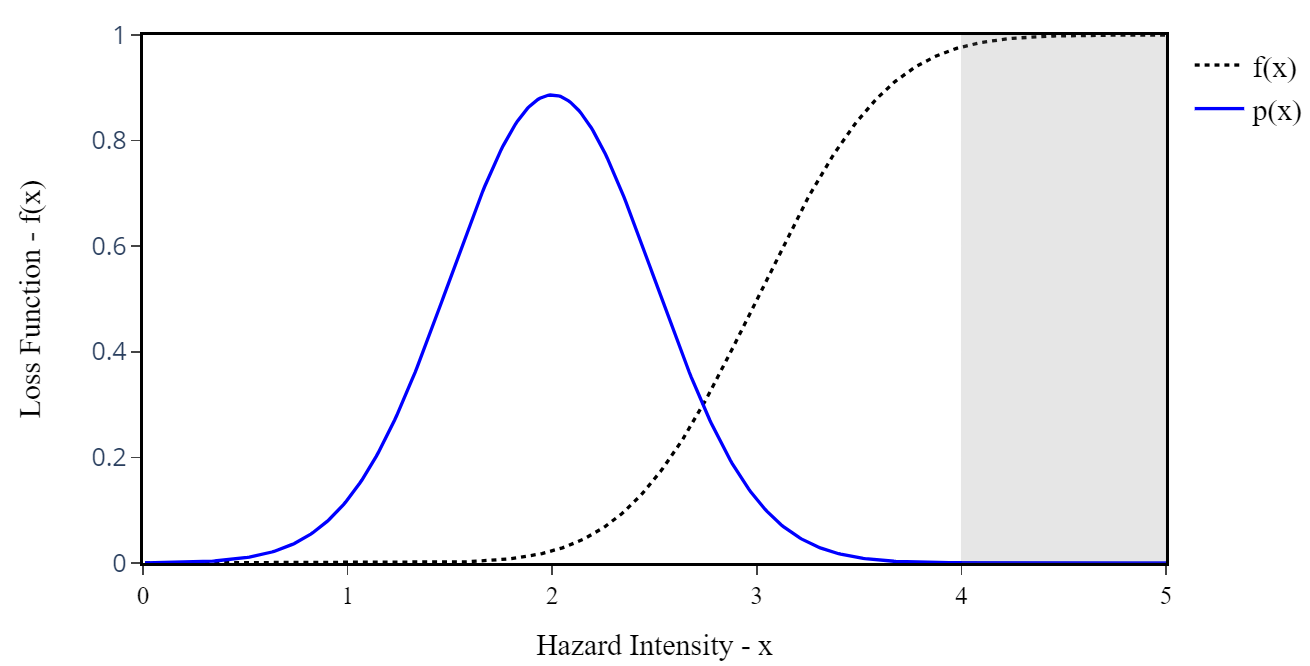
\includegraphics[scale=0.5]{Figures/Images/Illustrative Example/f&p}
        \caption{The graphs of $f(x)$ and $p(x)$ along with highlighted important region}
        \label{fig:f&p}
    \end{figure}

    Figure \ref{fig:f&p} illustrates the probability distribution function, $p(x)$, alongside the loss function, $f(x)$, with a specific focus on the shaded region representing the \textit{important area} where $f(x)$ exhibits higher values. \\
    The goal is to estimate the expected value of $f(x)$, a crucial metric in community resilience assessment. This expected value can be precisely determined by calculating the following integral:
    $$E[f(x)]=\int_{}^{}p(x)f(x)dx$$
    In this straightforward one-dimensional example, the integral can be readily computed as the area under the curve of $f(x)p(x)$ (depicted as the shaded region in Fig.~\ref{fig:true_value}) due to the problem's simplicity. \\
    The expected value, henceforth referred to as the "true-value," for this specific problem, has been precisely calculated as \TrueValue, as depicted in Fig.~\ref{fig:true_value}.
    
        \begin{figure}[H]
        \centering
        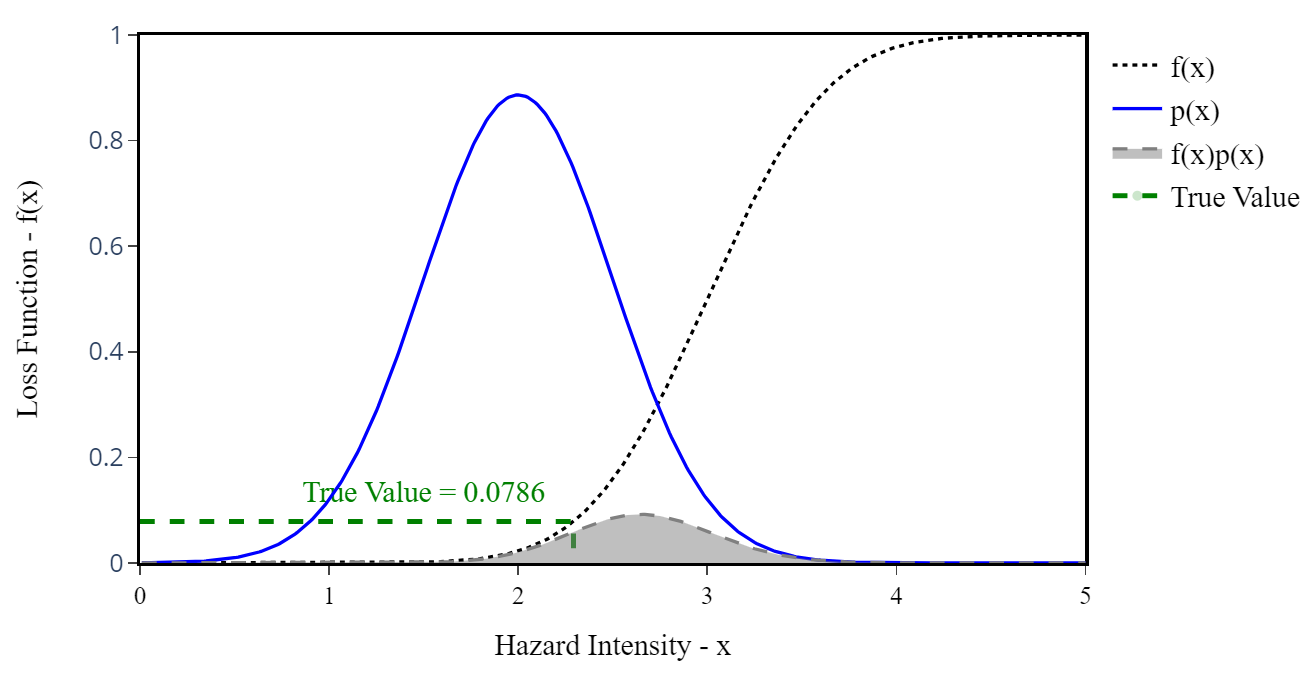
\includegraphics[scale=0.5]{Figures/Images/Illustrative Example/true_value.png}
        \caption{Calculation of the true value for the expected value of the function $f(x)$}
        \label{fig:true_value}
    \end{figure}

    However, in real-world applications characterized by multifaceted hazards and complex resilience actions, calculating the expected value becomes a formidable challenge. Consequently, simulation methods come into play. Here, the process of calculating the expected value of $f(x)$ using both MC simulation and IS methods is visually compared and differentiated.
    
    To estimate $E[f(x)]$ using the crude Monte Carlo method, we begin by sampling $x$ values from $p(x)$ and subsequently apply $f(x)$ to each of them. The average of these computed values yields an approximation of the expected value.\\ Fig.~\ref{fig:crude_MC_samples} demonstrates this process with \SampleSize{} samples, deliberately keeping the sample size small given the problem's simplicity. For the sake of fair comparison, a sample size of \SampleSize{} is maintained across all sampling methods.\\

        \begin{figure}[H]
        \centering
        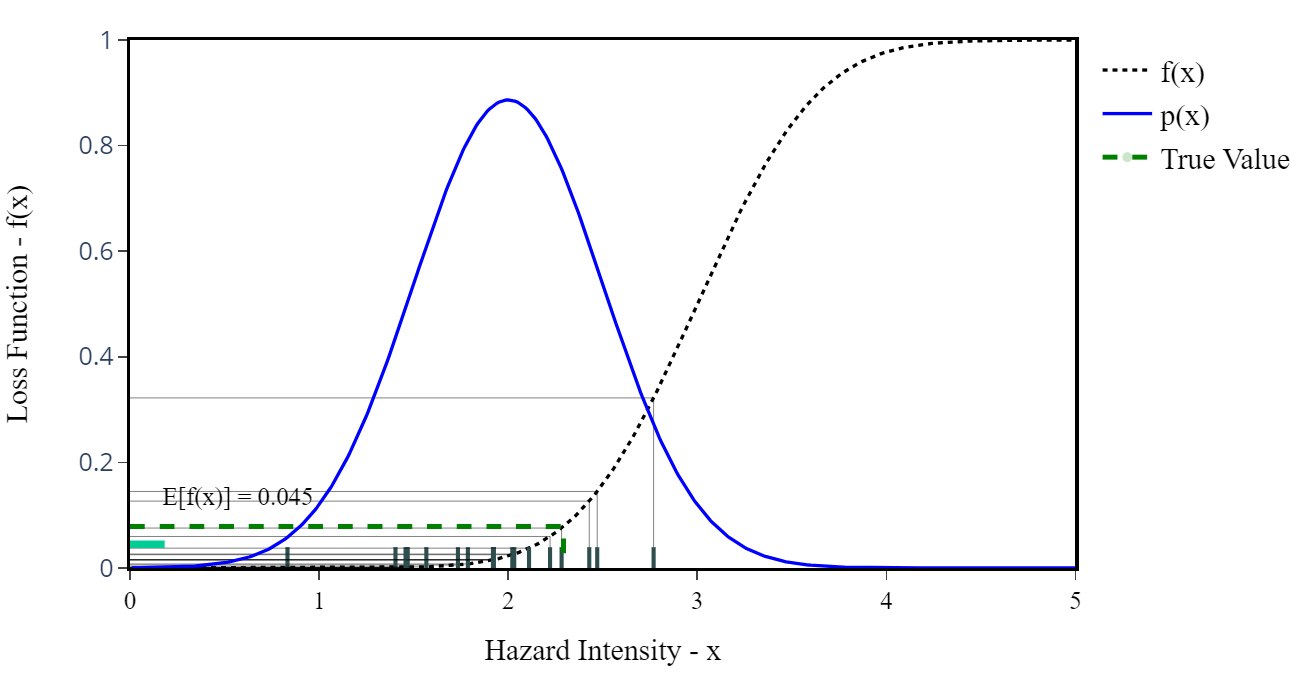
\includegraphics[scale=0.5]{Figures/Images/Illustrative Example/crude_MC_samples.png}
        \caption{Crude MC samples and their estimated expected value ($E[f(x)]$)}
        \label{fig:crude_MC_samples}
    \end{figure}

    As depicted in Fig.~\ref{fig:crude_MC_samples}, the majority of samples are generated from the high-probability, low-consequence region, leading to an underestimation of the expected value. Furthermore, the MC estimation results in a value of \MCResult. Although this value is not an exact match, it is relatively close to the true value of \TrueValue, as computed for this specific problem. This visualization provides insight into how MC simulation approximates the expected value of $f(x)$ by randomly sampling from the probability distribution.
    
    % When dealing with natural hazards, there may be a specific interest in worst-case scenarios, typically located in the tail of the probability distribution $p(x)$. To explore this approach, samples were generated from a truncated version of $p(x)$, where $x\geq 3$. The implementation of this method is visually represented in Fig.~\ref{fig:truncated_MC_samples}.
    
    %     \begin{figure}[H]
        \centering
        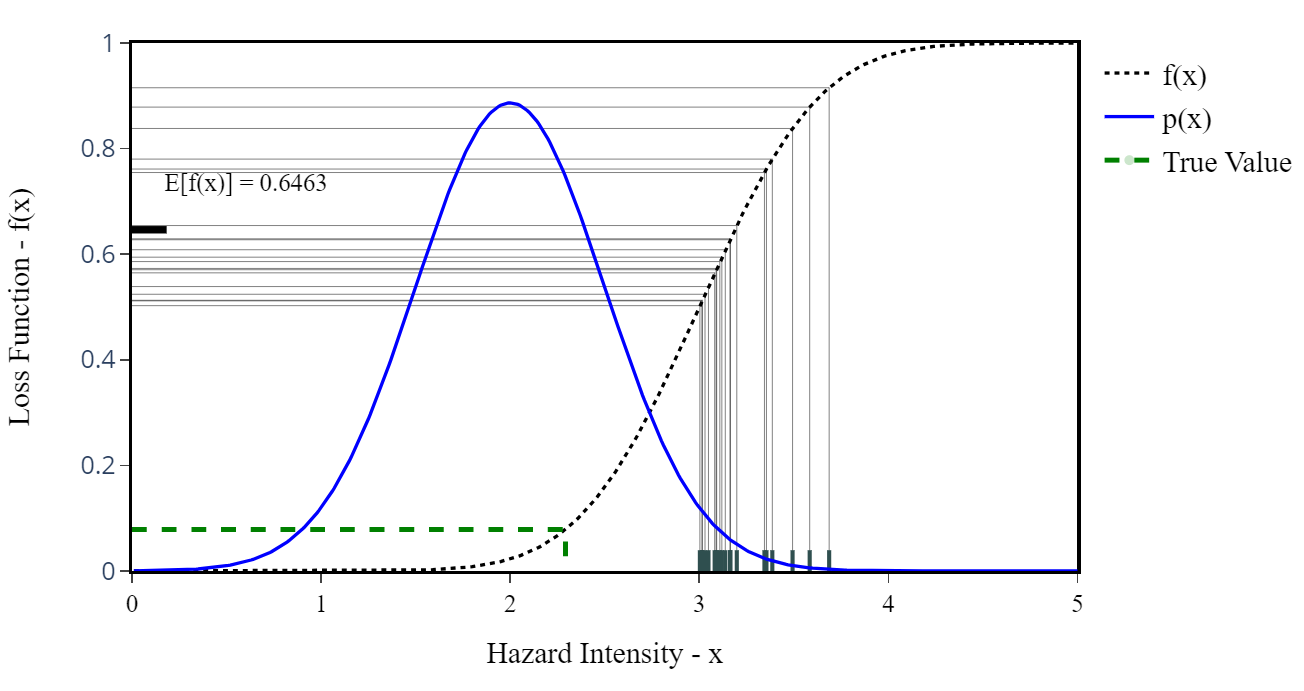
\includegraphics[scale=0.5]{Figures/Images/Illustrative Example/truncated_MC_samples.png}
        \caption{Generated samples from truncated MC along with the calculated $E[f(x)]$}
        \label{fig:truncated_MC_samples}
    \end{figure}

    % In this implementation, the expected value of $f(x)$ is estimated to be \TruncatedMCResult. Notably, it becomes evident that this estimated expectation value significantly deviates from the actual expectation value (\TrueValue). This observation underscores the potential drawbacks of designing exclusively for worst-case scenarios, which can lead to overestimation and unnecessary expenditure in resilience planning and action.

    To implement the importance sampling method, a new probability distribution, denoted as $q(x)$, is introduced as the importance density function. As previously mentioned, a common approach to selecting the importance density function involves retaining the same family of distribution as the original but adjusting its parameters. In the context of this one-dimensional problem, it becomes evident that the mean value of the original distribution, represented by $p(x)$, should be shifted to the right to generate more important samples with greater frequency. Fig.~\ref{fig:IS_dist} illustrates the importance distribution $q(x)$ and compares it with the original distribution, $p(x)$. 
    
        \begin{figure}[H]
        \centering
        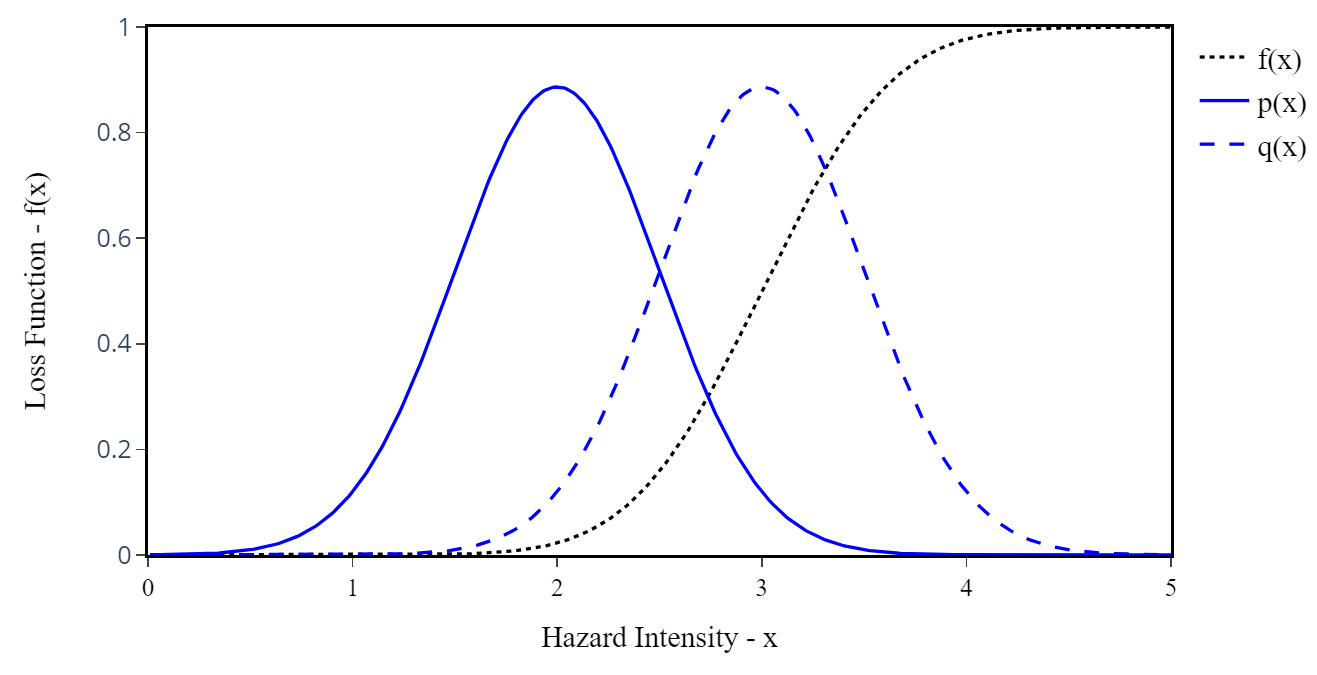
\includegraphics[scale=0.5]{Figures/Images/Illustrative Example/IS_dist.png}
        \caption{Importance Sampling distribution, strategically shifted towards high-consequence areas}
        \label{fig:IS_dist}
    \end{figure}
    
    To correct the bias introduced by this adjustment, we must modify the function $f(x)$ by applying a weighting factor equal to $\frac{p(x)}{q(x)}$. The importance distribution, along with the \SampleSize{} generated samples from it, is visually represented in Fig.~\ref{fig:IS_samples}.
    
        \begin{figure}[H]
        \centering
        \includegraphics[scale=0.5]{Figures/Images/Illustrative Example/IS_samples.png}
        \caption{Importance sampling distribution along with generated samples and the calculated $E[f(x)]$}
        \label{fig:IS_samples}
    \end{figure}

    In Fig.~\ref{fig:IS_samples}, the expected value of $f(x)$, computed using traditional IS, is calculated as \TraditionalISResult{}. Notably, with the same sample size as MC, IS has demonstrated the ability to estimate the expected value with reduced error. Nevertheless, it becomes apparent that addressing complex problems effectively necessitates a more systematic and universally applicable approach to determining the importance density function, rather than relying on manual adjustments, such as shifting it to the right or left.

    While various distributions can serve as an importance density function, an optimal importance density exists, capable of yielding MC estimates with zero variance \cite{asmussen_stochastic_2007}. The mathematical expression for this optimal importance density function is as follows:
    
    $$q^*=\frac{f(x)p(x)}{\int f(x)p(x)dx}$$

    Here, $q^{*}$ represents the optimal importance density function.

    In real-world applications, directly determining the expression mentioned above is challenging due to the unknown value of $\int{f(x)}{p(x)}dx$. However, in this example, where we possess knowledge of the actual integral value, we can compute the optimal importance density, illustrated as $q^*(x)$ in Fig.~\ref{fig:opt_IS_dist}.

        \begin{figure}[H]
        \centering
        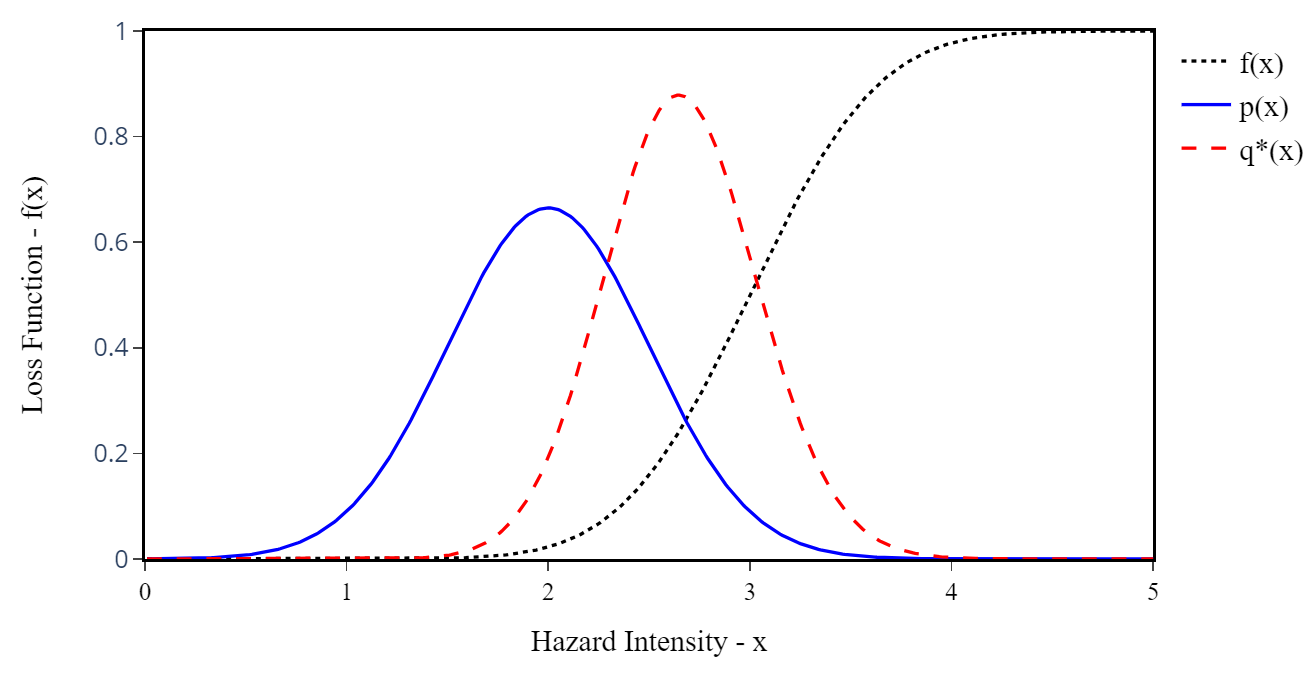
\includegraphics[scale=0.5]{Figures/Images/Illustrative Example/opt_IS_dist.png}
        \caption{Original probability distribution along with the optimum importance density function}
        \label{fig:opt_IS_dist}
    \end{figure}
    
    As previously mentioned, MCMC-IS serves as the method employed in this paper to approximate the optimal importance density function. The implementation of MCMC-IS is illustrated in two separate steps. In Fig.~\ref{fig:near_opt_IS_dist}, the process of generating MCMC samples using the Metropolise-Hasting algorithm and fitting a KDE to these samples is displayed. This initial step is pivotal in establishing a well-fitted probability density function that closely approximates the optimal importance density function. It's noteworthy that the number of generated MCMC samples in this phase is deliberately chosen to be sufficiently large, ensuring that the resulting KDE is a precise match to the optimal importance density function.

        \begin{figure}[H]
        \centering
        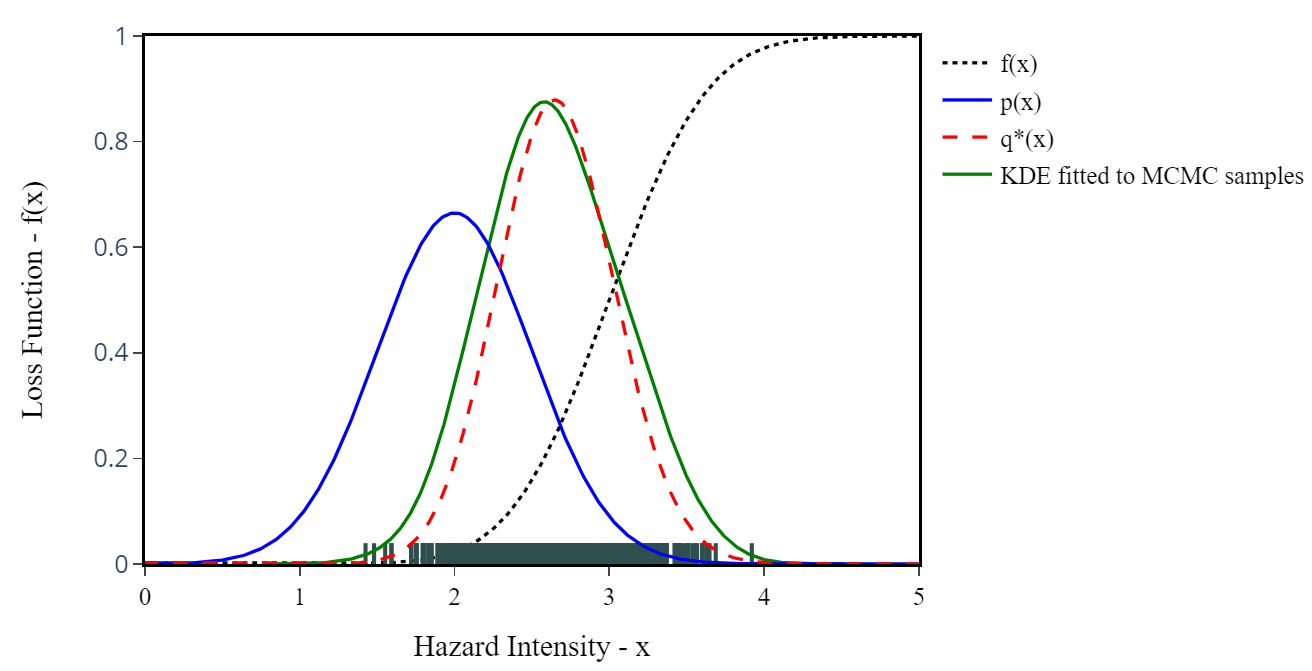
\includegraphics[scale=0.5]{Figures/Images/Illustrative Example/near_opt_IS_dist.png}
        \caption{Approximating the near-optimal importance sampling density function using MCMC-IS technique}
        \label{fig:near_opt_IS_dist}
    \end{figure}

    Once the well-fitted KDE is obtained, a new set of samples can be generated from the fitted KDE. Notably, the number of samples generated from the KDE doesn't need to be large. Even a small number of samples generated from the nearly optimal importance density function can provide an accurate estimate of the loss function. To eliminate the bias introduced by using q(x), the loss function is multiplied by the weighting factor as follows:

    $$weight=f(x)p(x)/kde.evaluate(x)$$

    Where, $kde.evaluate(x)$ represents the probability of $x$ as evaluated from the resulting KDE.
    
    The weighted function, in conjunction with the 20 samples generated from the fitted KDE and the resulting estimation from the MCMC-IS method, is depicted in Fig.~\ref{fig:MCMC_IS_samples}.
    
        \begin{figure}[H]
        \centering
        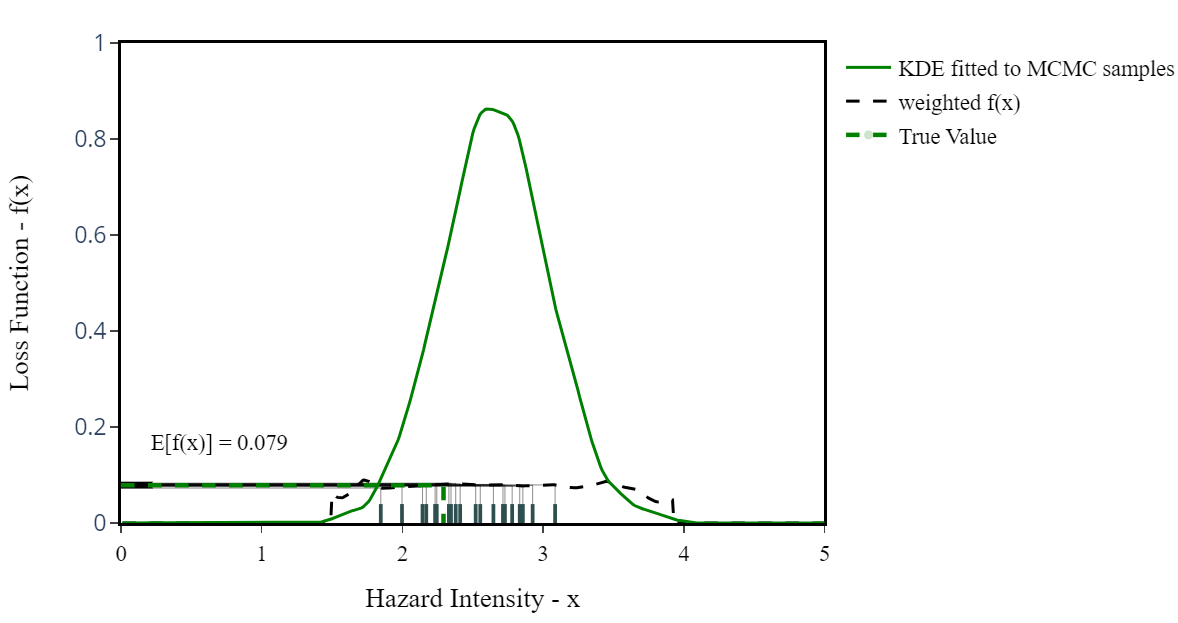
\includegraphics[scale=0.5]{Figures/Images/Illustrative Example/MCMC_IS_samples.png}
        \caption{Approximating the near-optimal importance sampling density function using MCMC-IS technique}
        \label{fig:MCMC_IS_samples}
    \end{figure}
    
    Fig.~\ref{fig:MCMC_IS_samples} illustrates that the MCMC-IS estimation, even with a small sample size, closely approximates the true value, showcasing the method's accuracy.
    
    In the concluding analysis of this section, the performance of three different estimation methods is compared, each evaluated against the true value of the problem's expected value, which stands at \TrueValue. The estimations and the relative error generated by the crude MC method, manual-IS, and MCMC-IS method are displayed in Table~\ref{table:illustrative_results}. It should be mentioned that to enhance the reliability of our results, we conducted each simulation method 10 times, calculating the average outcomes from these experiments. This strategy helps reduce the impact of random variability inherent in simulation techniques, providing a more dependable performance estimate.\\
        
    \begin{table}[H]
    \centering
    \caption{Comparison of estimation and relative error for three estimators in the illustrative example using 20 samples (Averaged over 10 experiments)}
    \label{table:illustrative_results}
    \small
    \begin{tabular}{lccc}
        \hline
        & \textbf{crude MC} & \textbf{manual-IS} & \textbf{MCMC-IS} \\
        \hline
        \textbf{Estimation}\\
        true value = \TrueValue & \MCResult & \TraditionalISResult & \MCMCISResult \\
        \textbf{Relative Error} & \MCError & \TraditionalISError & \MCMCISError\\
        \textbf{Standard Error of the Mean} & \MCSEM & \TraditionalISSEM & \MCMCISSEM\\
        \hline
    \end{tabular}
\end{table}

    The relative error measures the percentage difference between the estimated value and the true value, providing a clear indication of how close the estimation is to the actual result. In addition to the relative error, the standard error of the mean (SEM) is reported to quantify the statistical uncertainty in the estimates. The SEM represents the standard deviation of the sampling distribution of the mean, offering insights into the precision of the average estimate. Notably, the MCMC-IS approach demonstrates the most accurate estimation, closely followed by the manual-IS method, with the lowest SEM values indicating high precision. Conversely, the crude MC exhibits higher relative errors and SEM, indicating its limitation in accurately capturing the complex interplay of the loss function and probability distribution in this illustrative scenario. This comprehensive comparison provides invaluable insights into the strengths and weaknesses of each method, laying the groundwork for a detailed exploration in the subsequent sections.

        \begin{figure}[H]
        \centering
        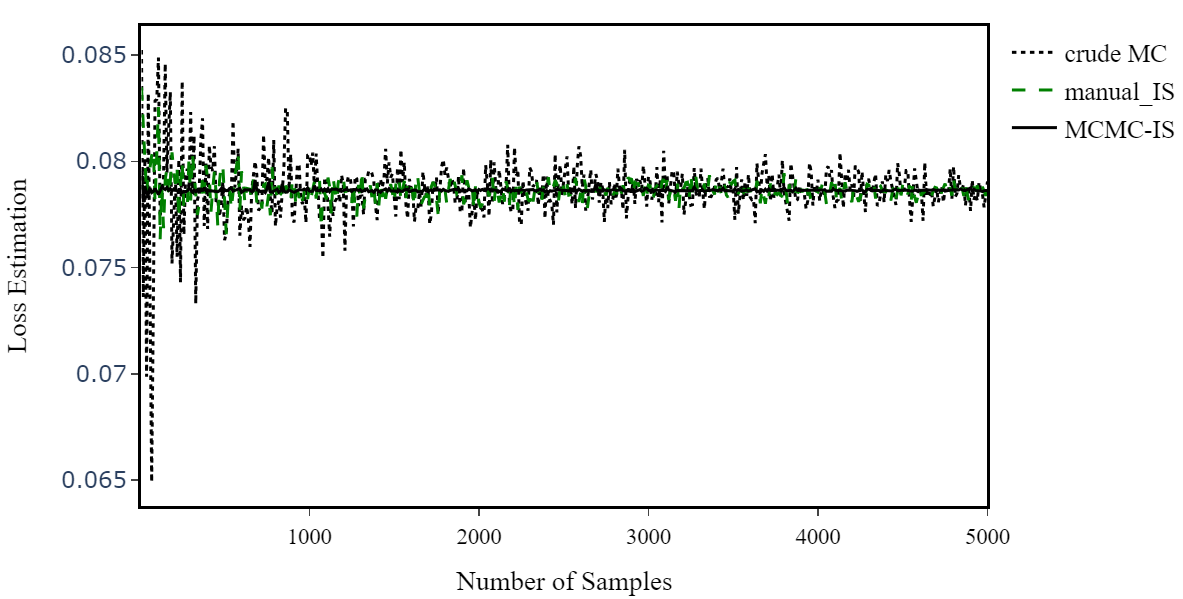
\includegraphics[scale=0.5]{Figures/Images/Illustrative Example/convergence_rate.png}
        \caption{Comparative convergence analysis of sampling methods}
        \label{fig:convergence_rate}
    \end{figure}
    
    Furthermore, Fig.~\ref{fig:convergence_rate} illustrates the convergence rates of each method with increasing sample size. Notably, MCMC-IS demonstrates exceptional convergence, approaching the true value rapidly even with a small sample size. This rapid convergence underscores the method’s efficiency in approximating the optimal importance density function.

    
        
        
